\pdfinfoomitdate=1
\pdftrailerid{}
\pdfsuppressptexinfo=15
\documentclass[10pt]{article}
\usepackage[letterpaper,margin=.65in]{geometry}
\usepackage[T1]{fontenc}
\usepackage{lmodern,microtype}
\usepackage{amsmath,amssymb,booktabs,array}
\usepackage{tikz}
\usetikzlibrary{calc}
\usepackage[hidelinks]{hyperref}
\hypersetup{pdftitle={Relative Polygonalization with Prescribed Traces: Two-page Summary},pdfauthor={Alec Kriebel}}
\setlength{\parindent}{0pt}
\setlength{\parskip}{.45em}
\newcommand{\code}{\operatorname{code}}
\title{\vspace{-2em}\bfseries Relative Polygonalization with Prescribed Traces\\[-.2em]
\large Two-page reader summary}
\author{Alec Kriebel\quad\textbar\quad Independent Researcher\quad\textbar\quad
\href{mailto:me@aleckriebel.com}{me@aleckriebel.com}}
\date{}
\begin{document}
\maketitle
\vspace{-2em}

\textbf{What a neural code records.}
Given open sets $U_1,\ldots,U_n$ in an ambient region, a point records the
indices of the sets containing it.  The collection of all such membership
patterns is the neural code.  When the fields are convex, code realizability
becomes a question about exact Venn-diagram geometry rather than metric
approximation.

\textbf{Known starting point.}
Bukh and Jeffs proved that every open convex code realizable in the plane has
a realization by interiors of convex polygons.  Their proof passes to
closures, selects a coordinatewise inclusion-minimal realization, and proves
that every member of a minimal planar tuple is polygonal.

\textbf{New relative theorem.}
Let $F$ be a compact convex polygon, let $U_1,\ldots,U_n$ be open convex
sets, choose finitely many affine lines, and choose finitely many atom
witnesses in $\operatorname{int}F$.  There are convex polygons $P_i$ such
that their interiors:
\begin{enumerate}
\item realize exactly the same code inside $\operatorname{int}F$;
\item have exactly the same trace on every prescribed line after clipping by
      $F$;
\item retain the corresponding closed line sections as well;
\item leave every protected witness in its original atom.
\end{enumerate}
The relative-affine statement also holds for segment and point carriers.

\begin{center}
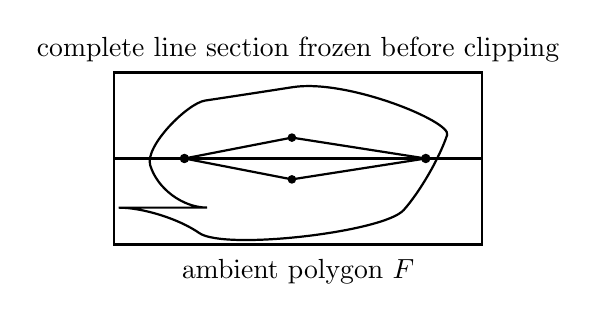
\begin{tikzpicture}[scale=.78]
  \draw[thick] (-3,-1.4) rectangle (3,1.4);
  \draw[thick,rounded corners=16pt] (-2.2,-.8) .. controls (-1.2,-1.5) and (1.4,-1.2) .. (2.2,-.3)
    .. controls (2.5,.6) and (.8,1.3) .. (-.8,1.05)
    .. controls (-1.8,.9) and (-2.5,.2) .. cycle;
  \draw[very thick] (-3,0)--(3,0);
  \fill (-1.85,0) circle (2.2pt); \fill (2.08,0) circle (2.2pt);
  \fill (-.1,.34) circle (2pt); \fill (-.1,-.34) circle (2pt);
  \draw[thick] (-1.85,0)--(-.1,.34)--(2.08,0)--(-.1,-.34)--cycle;
  \node[below] at (0,-1.48) {ambient polygon $F$};
  \node[above] at (0,1.42) {complete line section frozen before clipping};
\end{tikzpicture}
\end{center}

\textbf{Proof mechanism.}
For each nonempty strict line section $(a,b)$, retain a quadrilateral whose
diagonal is the closed section $[a,b]$.  Every point of $(a,b)$ remains
interior after shrinking, while $a$ and $b$ cannot move.  Tangent points and
supporting segments with empty strict trace are retained by their extreme
points.  Small triangles protect open-code words and designated witnesses;
all vertices of $F$ protect the ambient polygon.  The inclusion-minimal
planar argument then produces polygons while preserving this finite package.

\newpage
\textbf{Why recording the uncut section matters.}
If the bounded source section is $(a,b)$ and $F\cap L=[c,d]$, the relative
trace is
\[
 (a,b)\cap[c,d].
\]
It may be open, half-open, closed, a point, or empty.  Freezing $(a,b)$
first preserves the distinction between a source endpoint and an ambient
endpoint.  Literal endpoint equality also preserves simultaneous events for
several neurons.

\textbf{Coherent interfaces.}
If two planar face problems share an edge and inherit the same source trace,
applying the theorem to both faces produces polygonal models whose strict
memberships agree pointwise on that edge.  Endpoint positions, tangent
contacts, and simultaneous events agree as well.

\begin{center}
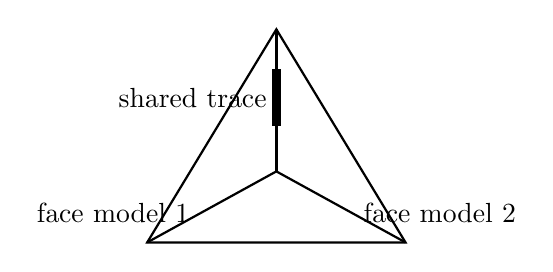
\begin{tikzpicture}[scale=.82]
  \coordinate (A) at (0,2.3); \coordinate (B) at (-2,-1); \coordinate (C) at (2,-1); \coordinate (D) at (0,.1);
  \draw[thick] (A)--(B)--(C)--cycle; \draw[thick] (A)--(D)--(B); \draw[thick] (D)--(C);
  \draw[very thick] (A)--(D);
  \draw[line width=3pt] ($(A)!.28!(D)$)--($(A)!.68!(D)$);
  \node[left] at ($(A)!.48!(D)$) {shared trace};
  \node[below left] at (-1.2,-.25) {face model 1};
  \node[below right] at (1.2,-.25) {face model 2};
\end{tikzpicture}
\end{center}

\textbf{Tetrahedral-boundary application.}
Choose four affinely independent source witnesses and record the complete
interval trace of every neuron on all six edges of their tetrahedron.  Apply
the relative theorem to each triangular face, prescribing its three edge
lines.  The resulting four face models agree on all six shared edges, giving
a coherent finite polygonal model of the complete boundary sphere.

\textbf{Exact limitation.}
The theorem controls planar codes and finitely many one-dimensional
membership traces.  It does not match numerical defining functions or
normal derivatives across an edge, and it does not provide a convex
three-dimensional filling of the tetrahedral boundary.

\textbf{Reproducibility.}
A deterministic exact-rational package checks generic, tangent, point,
half-open, simultaneous, lower-dimensional, covered-carrier, shared-edge,
and tetrahedral-boundary examples.  These are regression tests; the general
theorem is geometric.
\end{document}
